
\begin{center}
\section{Clases prácticas}
\end{center}

{\raggedright
\subsection{Actividad 5 en clase}
}\vspace{.5cm}

\textbf{Desarrolla los siguientes programas en clase.}\vspace{.2mm}

\begin{itemize}
\item \textbf{Programa 1:} Hilo de nombres con metodo sleep y random.
\item \textbf{Programa 2:} Hilo con método for y con método yield.
\item \textbf{Programa 3:} Interfaz y funcionamiento de una calculadora con metodo join y validación de datos.
\end{itemize}\vspace{.5cm}

\textbf{\textit{Solución del primer programa.}}

\begin{center}
Clase Hilo1.java
\end{center}

\begin{verbatim}
public class Hilo1 extends Thread{
    
    String nombres;
    
    public Hilo1(String nombre){
        this.nombres=nombre;
    }
    
    @Override
    public void run(){
        int x = (int) (Math.random()*3000);
        try{
            Thread.sleep(x);
            System.out.println("Soy: "+nombres+", durmió "+x);
        }catch(InterruptedException ex){
            System.out.println("Error hilo: "+ex.getMessage());
        }
    }
}
\end{verbatim} \vspace{1cm}

\begin{center}
Clase DiplomadosHilos.java (main)
\end{center}

\begin{verbatim}
public class DiplomadosHilos {

    public static void main(String[] args) {
        // TODO code application logic here
        Hilo1 h1 = new Hilo1("Saul");
        Hilo1 h2 = new Hilo1("Karen");
        Hilo1 h3 = new Hilo1("Carlos");
        
        h1.start();
        h2.start();
        h3.start();
        System.out.println("Corriendo hilos");
    }
    
}
\end{verbatim} \vspace{1cm}
\begin{figure}[h!]
		\centering
		{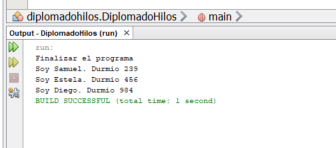
\includegraphics[scale=1.5]{40.jpg}\par} 
		\caption{Salida del primer programa, Actividad 5}\vspace{1cm}
\end{figure}

\textbf{\textit{Solución del segundo programa.}}

\begin{center}
Clase DiplomadosHilos2.java (main)
\end{center}

\begin{verbatim}
public class DiplomadosHilos2 {

    public static void main(String[] args) {
        // TODO code application logic here
        ElHilo h1 = new ElHilo("Saul");
        ElHilo h2 = new ElHilo("Naranja");
        
        h1.start();
        h2.start();
    }

    static class ElHilo extends Thread {
        String nombre;

        public ElHilo(String nombre) {
            this.nombre = nombre;
        }

        public void run() {
            for (int i = 0; i < 6; i++) {
                System.out.println("nombre es: " + nombre + " / " + i);
                yield();
            }
        }
    }
}
\end{verbatim} \vspace{1cm}
\begin{figure}[h!]
		\centering
		{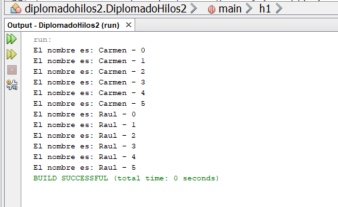
\includegraphics[scale=1.5]{41.jpg}\par} 
		\caption{Salida del segundo programa, Actividad 5}\vspace{1cm}
\end{figure}

\textbf{\textit{Solución del tercer programa.}}

\begin{center}
Clase Multiplicacion.java
\end{center}

\begin{verbatim}
public class Multiplicacion extends Thread{
    int a,b,r;

    public Multiplicacion(Integer a, Integer b) {
        this.a = a;
        this.b = b;
    }
    
    @Override
    public void run(){
        
        r = a*b;
        System.out.println("La multiplicacion es: "+r);
    }
}
\end{verbatim} \vspace{1cm}

\begin{center}
Clase Resta.java
\end{center}

\begin{verbatim}
public class Resta extends Thread{
    int a,b,r;

    public Resta(Integer a, Integer b) {
        this.a = a;
        this.b = b;
    }
    
    @Override
    public void run(){
        
        r = a-b;
        System.out.println("La resta es: "+r);
    }
}
\end{verbatim} \vspace{1cm}

\begin{center}
Clase Suma.java
\end{center}

\begin{verbatim}
public class Suma extends Thread{
    int a,b,r;

    public Suma(Integer a, Integer b) {
        this.a = a;
        this.b = b;
    }
    
    @Override
    public void run(){
        
        r = a+b;
        System.out.println("La suma es: "+r);
    }
}
\end{verbatim} \vspace{1cm}

\begin{center}
Clase Calculadora.java (main)
\end{center}

\begin{verbatim}
public class Calculadora extends javax.swing.JFrame {
    public Calculadora() {
        initComponents();
    }
    private void salirActionPerformed(java.awt.event.ActionEvent evt) {                                      
        // TODO add your handling code here:
        System.exit(0);
    }                                     

    private void iniciarActionPerformed(java.awt.event.ActionEvent evt) {                                        
        // TODO add your handling code here:

        int a, b;
        a = Integer.parseInt(valor1.getText());
        b = Integer.parseInt(valor2.getText());
        Suma s = new Suma(a, b);
        Resta r = new Resta(a, b);
        Multiplicacion m = new Multiplicacion(a, b);

        System.out.println("a= " + a);
        System.out.println("b= " + b);

        s.start();
        r.start();
        m.start();

        try {
            s.join();
            r.join();
            m.join();
        } catch (InterruptedException ex) {
            Logger.getLogger(Calculadora.class.getName()).log(Level.SEVERE, null, ex);
        }

        resultadoSuma.setText(String.valueOf(s.r));
        resultadoResta.setText(String.valueOf(r.r));
        resultadoMultiplicacion.setText(String.valueOf(m.r));
    }
    public boolean validar(String numero) {
        int n;
        try {
            n = Integer.parseInt(numero);
            return true;
        } catch (Exception e) {
            System.out.println("Error: " + e.getMessage());
            return false;
        }
    }

}
\end{verbatim} \vspace{1cm}
\begin{figure}[h!]
		\centering
		{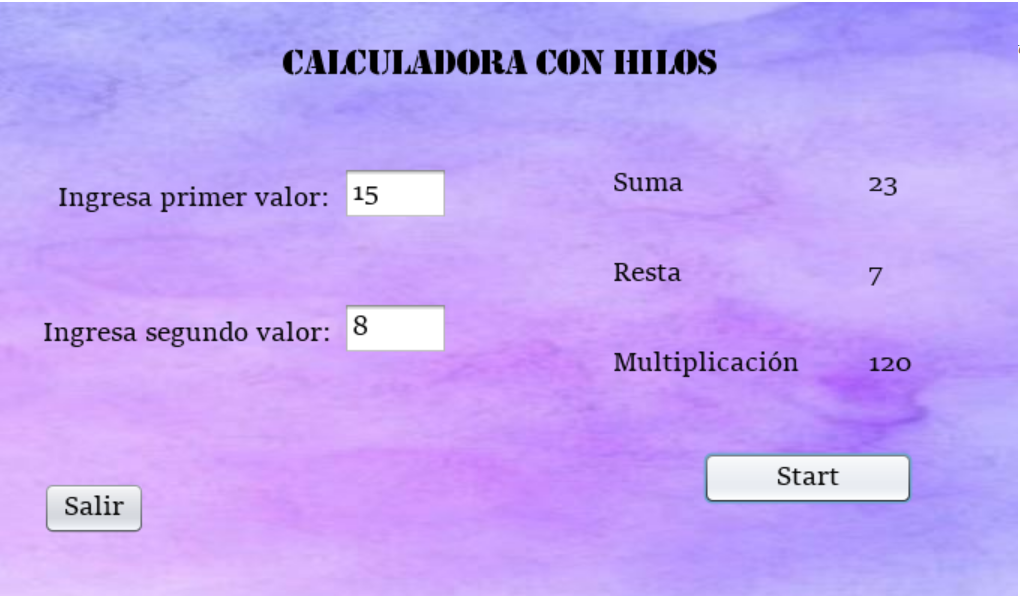
\includegraphics[scale=.7]{42.jpg}\par} 
		\caption{Salida del tercer programa, Actividad 5}\vspace{1cm}
\end{figure}

{\raggedright
\subsection{Actividad 6 en clase}
}\vspace{.5cm}

\textbf{Desarrolla los siguientes programas en clase.}\vspace{.2mm}

\begin{itemize}
\item \textbf{Programa 1:} Formas de instanciar un hilo.
\item \textbf{Programa 2:} Bola magica.
\item \textbf{Programa 3:} Grupo Procesos.
\end{itemize}\vspace{.5cm}

\textbf{\textit{Solución del primer programa.}}

\begin{center}
Clase hilos.java
\end{center}

\begin{verbatim}
public class hilos implements Runnable{ 
    private String mensaje;
    
    public hilos(String m){
        this.mensaje=m;
    }

    public void run(){
        System.out.println("hola for interno: "+mensaje);
        dormirmensaje();
    }
    
    private void dormirmensaje(){
        try {
            Thread.sleep(2000);
        } catch (InterruptedException e) {
            e.printStackTrace();
        }
    }
}
\end{verbatim} \vspace{1cm}

\begin{center}
Clase FormasdeInstanciarHilos.java (main)
\end{center}

\begin{verbatim}
public class FormasdeInstanciarHilos {

    public static void main(String[] args) {
        // TODO code application logic here
        ExecutorService executor = Executors.newFixedThreadPool(5);
        for (int i = 0; i < 10; i++) {
            Runnable h=new hilos("for externo: "+i);
            executor.execute(h);
        }
        executor.shutdown();
        while(!executor.isTerminated()){
        }
        System.out.println("Finaliza hilos");
    }
}
\end{verbatim} \vspace{1cm}
\begin{figure}[h!]
		\centering
		{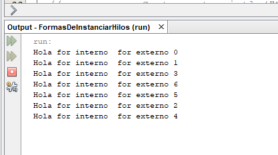
\includegraphics[scale=1.5]{43.jpg}\par} 
		\caption{Salida del primer programa, Actividad 6}\vspace{1cm}
\end{figure}\newpage

\textbf{\textit{Solución del segundo programa.}}

\begin{center}
Clase FraseAmor.java
\end{center}

\begin{verbatim}
public class FraseAmor extends Thread{
    String frase;
    
    public void run(){
        int caso=(int)(Math.random()*5);
        
        switch(caso){
            case 1: frase="Echale ganas a tu trabajo";
                break;
            case 2: frase="Trabaja duro todos los dias";
                break;
            case 3: frase="Nunca renuncies a tus sueños";
                break;
            case 4: frase="Conoce gente nueva en tu trabajo";
                break;
            case 5: frase="Comparte conocimientos";
                break;
            default:  frase="Amor...";
        }
    }
}
\end{verbatim} \vspace{1cm}

\begin{center}
Clase FraseTrabajo.java
\end{center}

\begin{verbatim}
public class FraseTrabajo extends Thread{
    String frase;
    
    public void run(){
        int caso=(int)(Math.random()*5);
        
        switch(caso){
            case 1: frase="Amate a ti mismo";
                break;
            case 2: frase="Ama a los que te rodean";
                break;
            case 3: frase="Ama todo lo que haces";
                break;
            case 4: frase="Vendran cosas nuevas en tu vida";
                break;
            case 5: frase="Nunca te rindas";
                break;
            default:  frase="Trabajo...";
        }
    }
    
}
\end{verbatim} \vspace{1cm}

\begin{center}
Clase frasebolamagica.java (main)
\end{center}

\begin{verbatim}
public class frasebolamagica extends javax.swing.JFrame {
    private void btnSalirActionPerformed(java.awt.event.ActionEvent evt) {                                         
        // TODO add your handling code here:
        System.exit(0);
    }                                        

    private void btnIniciarActionPerformed(java.awt.event.ActionEvent evt) {                                           
        // TODO add your handling code here:
        FraseTrabajo t= new FraseTrabajo();
        FraseAmor a= new FraseAmor();
        t.start();
        a.start();
        try {
            t.join();
            a.join();
        } catch (InterruptedException ex) {
            Logger.getLogger(frasebolamagica.class.getName()).log(Level.SEVERE, null, ex);
        }
        frase1.setText(t.frase);
        frase2.setText(a.frase);
        
    }
}
\end{verbatim} 
\begin{figure}[h!]
		\centering
		{
\includegraphics[scale=.43]{44.jpg}\par} 
		\caption{Salida del segundo programa, Actividad 6}\vspace{1cm}
\end{figure}

\textbf{\textit{Solución del tercer programa.}}

\begin{center}
Clase Hilo1.java
\end{center}

\begin{verbatim}
public class Hilo1 extends Thread{
    int limite, Timesleep;

    public Hilo1(int limite, int Timeslepp) {
        this.limite = limite;
        this.Timesleep=Timesleep;
    }
    
    public void run(){
        for (int i = 0; i < limite; i++) {
            System.out.println("Hilo1: "+i);
            dormir();
        }
    }
    
    public void dormir(){
        try {
            Hilo1.sleep(Timesleep);
        } catch (InterruptedException ex) {
            System.out.println("Error"+ex.getMessage());
        }
    }
}
\end{verbatim} \vspace{1cm}

\begin{center}
Clase Hilo2.java
\end{center}

\begin{verbatim}
public class Hilo2 implements Runnable{
    int limite, Timesleep;

    public Hilo2(int limite, int Timeslepp) {
        this.limite = limite;
        this.Timesleep=Timesleep;
    }
    
    public void run(){
        for (int i = 0; i < limite; i++) {
            System.out.println("Hilo2: "+i);
            dormir();
        }
    }
    
    public void dormir(){
        try {
            Thread.sleep(Timesleep);
        } catch (InterruptedException ex) {
            System.out.println("Error"+ex.getMessage());
        }
    }
}
\end{verbatim} \vspace{1cm}

\begin{center}
Clase Hilo3.java
\end{center}

\begin{verbatim}
public class Hilo3 extends Thread {
    int limite, Timesleep;

    public Hilo3(int limite, int Timeslepp) {
        this.limite = limite;
        this.Timesleep=Timesleep;
    }
    
    public void run(){
        for (int i = 0; i < limite; i++) {
            System.out.println("Hilo3: "+i+5);
            dormir();
        }
    }
    
    public void dormir(){
        try {
            Hilo3.sleep(Timesleep);
        } catch (InterruptedException ex) {
            System.out.println("Error"+ex.getMessage());
        }
    }
}
\end{verbatim} \vspace{1cm}

\begin{center}
Clase Prioridades.java (main)
\end{center}

\begin{verbatim}
public class Prioridades {

    public static void main(String[] args) {
        // TODO code application logic here
        Thread h1=new Thread(new Hilo1(10, 1000));
        Runnable h2=new Hilo2(5,500);
        Hilo3 h3=new Hilo3(6, 500);
        
        h3.start();
        h1.start();
        h2.run();
        
        h1.setPriority(10);//Maxima prioridad
        h1.setPriority(1);//Minima prioridad
        
    }
}
\end{verbatim} \vspace{1cm}
\begin{figure}[h!]
		\centering
		{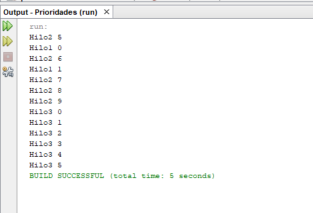
\includegraphics[scale=1.5]{45.jpg}\par} 
		\caption{Salida del tercer programa, Actividad 6}\vspace{1cm}
\end{figure}\newpage

{\raggedright
\subsection{Actividad 7 en clase}
}\vspace{.5cm}

\textbf{Desarrolla un cronometro con hilos, hilo segundos, hilo minutos con sincronización sleep.}\vspace{.2mm}

\textbf{\textit{Solución del programa.}}

\begin{center}
Clase Hilosegundos.java
\end{center}

\begin{verbatim}
public class Hilosegundos extends Thread {

    @Override
    public void run() {

        for (int i = 0; i < 60; i++) {
            for (int j = 0; j < 60; j++) {
                if (j < 10) {
                    System.out.println(":0" + j);
                } else {
                    System.out.println(j);
                }

                try {
                    Thread.sleep(1000);
                } catch (InterruptedException ex) {
                    System.out.println("Error sleep" + ex.getMessage());
                }
            }
        }
    }
}
\end{verbatim} \vspace{1cm}

\begin{center}
Clase Hilominutos.java
\end{center}

\begin{verbatim}
public class Hilominutos extends Thread {

    @Override
    public void run() {
        for (int i = 0; i < 60; i++) {
            for (int j = 0; j < 60; j++) {
                if (i < 10) {
                    System.out.print("0" + i);
                } else {
                    System.out.print(i);
                }

                try {
                    Thread.sleep(1000);
                } catch (InterruptedException ex) {
                    System.out.println("Error sleep" + ex.getMessage());
                }
            }
        }
    }
}
\end{verbatim} \vspace{1cm}

\begin{center}
Clase Cronometro.java (main)
\end{center}

\begin{verbatim}
public class Cronometro {

    public static void main(String[] args) {
        // TODO code application logic here
        Hilominutos h1=new Hilominutos();
        Hilosegundos h2=new Hilosegundos();
        
        h1.start();
        
        try {
            h1.sleep(50);
        } catch (InterruptedException ex) {
            System.out.println("Error sleep"+ ex.getMessage());
        }
        
        h2.start();
        try {
            h2.sleep(50);
        } catch (InterruptedException ex) {
            System.out.println("Error sleep"+ ex.getMessage());
        } 
    }
    
}
\end{verbatim} \vspace{1cm}

\begin{figure}[h!]
		\centering
		{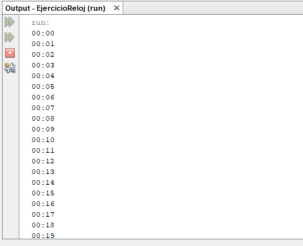
\includegraphics[scale=1.5]{46.jpg}\par} 
		\caption{Salida del programa, Actividad 7}\vspace{1cm}
\end{figure}\newpage

{\raggedright
\subsection{Actividad 8 en clase}
}\vspace{.5cm}

\textbf{Desarrolla los siguientes programas en clase.}\vspace{.2mm}

\begin{itemize}
\item \textbf{Programa 1:} GUI cronometro con horas, min, seg. Clase Observable.
\item \textbf{Programa 2:} Paso de parametros.
\item \textbf{Programa 3:} Sincronización con sleep.
\end{itemize}\vspace{.5cm}

\textbf{\textit{Solución del primer programa.}}

\begin{center}
Clase RelojHilosObserver.java
\end{center}

\begin{verbatim}
public class RelojHilosObserver extends Observable implements Runnable {

    int horas, min, seg;

    public RelojHilosObserver(int horas, int min, int seg) {
        this.horas = horas;
        this.min = min;
        this.seg = seg;
    }

    @Override
    public void run() {
        String t;
        //horas
        while (true) {
            t = "";//para colocar los : en cada separacion y de inicio en poner cero
            //horas
            if (horas < 10) {
                t += "0" + horas;
            } else {
                t += horas;
            }
            t += ":";
            //minutos
            if (min < 10) {
                t += "0" + min;
            } else {
                t += min;
            }
            t += ":";
            //segundos
            if (seg < 10) {
                t += "0" + seg;
            } else {
                t += seg;
            }
            seg++;
            if (seg == 60) {
                min++;
                seg = 0;
                if (min == 60) {
                    min = 0;
                    horas++;
                    if (horas == 24) {
                        horas = 0;
                    }
                }
            }
            
            try {
                Thread.sleep(1000);
            } catch (InterruptedException ex) {
                System.out.println("Error dormir hilo"+ex.getMessage());
            }
            //colocamos observable
            this.setChanged();
            this.notifyObservers(t);
            this.clearChanged();
        }
    }
}
\end{verbatim} \vspace{1cm}

\begin{center}
Clase relojhilos.java (main)
\end{center}

\begin{verbatim}
public class relojhilos extends javax.swing.JFrame implements Observer{
    private void btnIniciarActionPerformed(java.awt.event.ActionEvent evt) {                                           
        // TODO add your handling code here:
        this.btnIniciar.setEnabled(false);
        RelojHilosObserver r = new RelojHilosObserver(10,10,40);
        r.addObserver(this);
        Thread t=new Thread(r);
        t.start();
    }                                          

    private void btnSalirActionPerformed(java.awt.event.ActionEvent evt) {                                         
        // TODO add your handling code here:
        System.exit(0);
    } 
		
    @Override
    public void update(Observable o, Object arg) {
        cronometro.setText((String)arg);
    }
}
\end{verbatim} \vspace{1cm}
\begin{figure}[h!]
		\centering
		{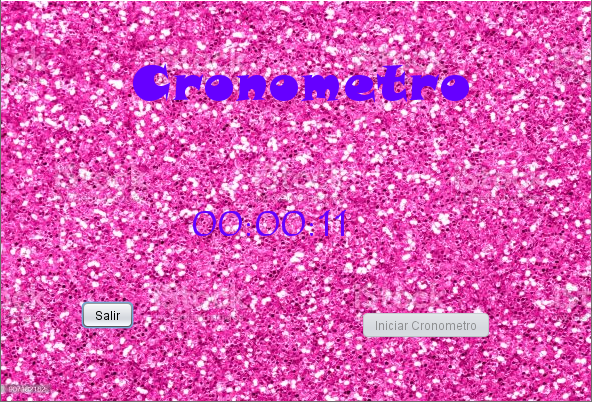
\includegraphics[scale=1.2]{47.jpg}\par} 
		\caption{Salida del primer programa, Actividad 8}\vspace{1cm}
\end{figure}

\textbf{\textit{Solución del segundo programa.}}

\begin{center}
Clase Hilo1.java
\end{center}

\begin{verbatim}
public class Hilo1 extends Thread{
    String nombre;
    int edad;

    public Hilo1(String nonmbre, int edad) {
        
        this.edad = edad;
        this.nombre = nombre;
    }
    
    @Override
    public void run(){
        System.out.println(nombre + " tiene " + edad + "años");
    }
}
\end{verbatim} \vspace{1cm}

\begin{center}
Clase Hilo2.java
\end{center}

\begin{verbatim}
public class Hilo2 extends Thread{
    String nombre;
    int edad;
    
    @Override
    public void run(){
        System.out.println(nombre + " tiene " + edad + "años");
    }
    
    public void datos(String nombre, int edad){
        this.edad = edad;
        this.nombre = nombre;
    } 
}
\end{verbatim} \vspace{1cm}

\begin{center}
Clase PasodeParametrosHilos.java (main)
\end{center}

\begin{verbatim}
public class PasodeParametrosHilos {

    public static void main(String[] args) {
        // TODO code application logic here

        Hilo1 h1 = new Hilo1("Sofia",22);//Paso parametros con constructor
        Hilo2 h2 = new Hilo2();
        h2.datos("Ivan",25);//paso parametros con metodo
        
        h1.start();
        h2.start();
    }
    
}
\end{verbatim} \vspace{1cm}
\begin{figure}[h!]
		\centering
		{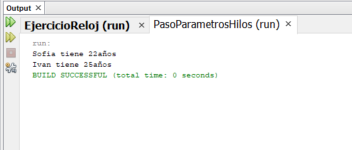
\includegraphics[scale=1.5]{48.jpg}\par} 
		\caption{Salida del segundo programa, Actividad 8}\vspace{1cm}
\end{figure}

\textbf{\textit{Solución del tercer programa.}}

\begin{center}
Clase Hilo1.java
\end{center}

\begin{verbatim}
public class Hilo1 extends Thread {

    @Override
    public void run() {
        for (int j = 0; j < 3; j++) {
            System.out.print("H");
            
            try {
                Thread.sleep(1000);
            } catch (InterruptedException ex) {
                System.out.println("Error sleep"+ ex.getMessage());
            }
          
        }
    }
}
\end{verbatim} \vspace{1cm}

\begin{center}
Clase Hilo2.java
\end{center}

\begin{verbatim}
public class Hilo2 extends Thread {

    @Override
    public void run() {
        for (int j = 0; j < 3; j++) {
            System.out.println(" i");
            try {
                Thread.sleep(1000);
            } catch (InterruptedException ex) {
                System.out.println("Error sleep"+ ex.getMessage());
            }
        }
    }
}
\end{verbatim} \vspace{1cm}

\begin{center}
Clase Sincronizacionsleephilos.java (main)
\end{center}

\begin{verbatim}
public class Sincronizacionsleephilos {

    public static void main(String[] args) {
        // TODO code application logic here
        Hilo1 h1=new Hilo1();
        Hilo2 h2=new Hilo2();
        
        h1.start();
        
        try {
            h1.sleep(50);
        } catch (InterruptedException ex) {
            System.out.println("Error sleep"+ ex.getMessage());
        }
        
        h2.start();
        try {
            h2.sleep(50);
        } catch (InterruptedException ex) {
            System.out.println("Error sleep"+ ex.getMessage());
        }      
    }
    
}
\end{verbatim} \vspace{1cm}
\begin{figure}[h!]
		\centering
		{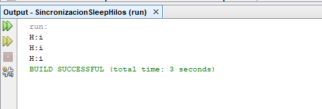
\includegraphics[scale=1.8]{49.jpg}\par} 
		\caption{Salida del tercer programa, Actividad 8}\vspace{1cm}
\end{figure}

{\raggedright
\subsection{Actividad 9 (Tarea)}
}\vspace{.5cm}

\textbf{Desarrolla un programa GUI carrera de canicas con Observable, dos hilos minimo.}\vspace{.2mm}

\textbf{\textit{Solución de la tarea.}}

\begin{center}
Clase Hilo1.java
\end{center}

\begin{verbatim}
public class Hilo1 extends Observable implements Runnable{
    int x, i;

    @Override
    public void run() {
        x = (int)(Math.random()*400);
        for (i = 490; i > x; i--) {
            try {
                System.out.println(i);
                sleep(7);
            } catch (InterruptedException ex) {
                Logger.getLogger(Hilo1.class.getName()).log(Level.SEVERE, null, ex);
            }
            this.setChanged();
            this.notifyObservers(i);
            this.clearChanged();
        }
    }
    
}
\end{verbatim} \newpage

\begin{center}
Clase Hilo2.java
\end{center}

\begin{verbatim}
public class Hilo2 extends Observable implements Runnable{
    int x, i;

    @Override
    public void run() {
        x = (int)(Math.random()*400);
        for (i = 510; i > x; i--) {
            try {
                System.out.println(i);
                sleep(7);
            } catch (InterruptedException ex) {
                Logger.getLogger(Hilo1.class.getName()).log(Level.SEVERE, null, ex);
            }
            this.setChanged();
            this.notifyObservers(i);
            this.clearChanged();
        }
    }
    
}
\end{verbatim} \vspace{1cm}

\begin{center}
Clase Carrera.java (main)
\end{center}

\begin{verbatim}
public class Carrera extends javax.swing.JFrame implements Observer{
    Hilo1 h1 = new Hilo1();
    Hilo2 h2 = new Hilo2();
    
    public Carrera() {
        initComponents();
        this.setLocationRelativeTo(null);
    }

    private void salirActionPerformed(java.awt.event.ActionEvent evt) {                                      
        // TODO add your handling code here:
        System.exit(0);
    }                                     

    private void iniciarActionPerformed(java.awt.event.ActionEvent evt) {                                        
        // TODO add your handling code here:
        Thread t = new Thread(h1);
        t.start();
        h1.addObserver(this);
        
        Thread t2 = new Thread(h2);
        t2.start();
        h2.addObserver(this);

    }              

    @Override
    public void update(Observable o, Object arg) {
        carro1.setLocation(100, (int) arg);
        carro2.setLocation(190, (int) h1.i);
    }
}
\end{verbatim} \vspace{1cm}
\begin{figure}[h!]
		\centering
		{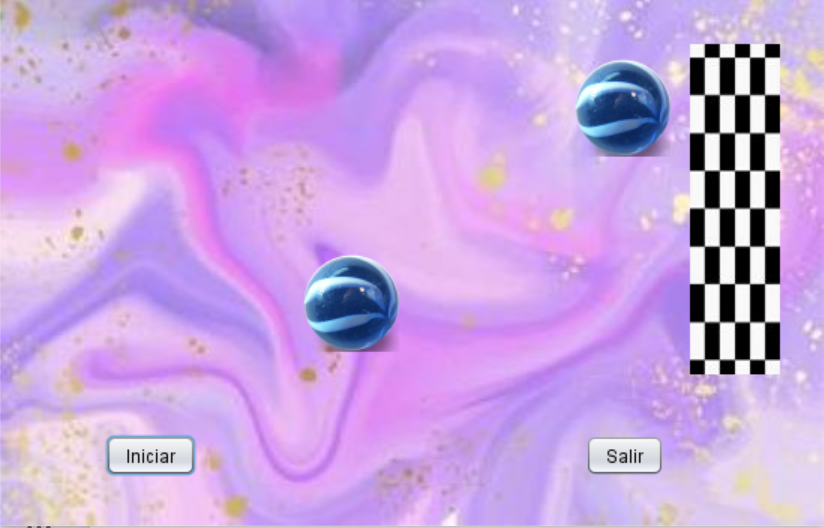
\includegraphics[scale=.7]{50.jpg}\par} 
		\caption{Salida del programa, Actividad 9 (Tarea)}\vspace{1cm}
\end{figure}\newpage

{\raggedright
\subsection{Actividad 10 en clase}
}\vspace{.5cm}

\textbf{Desarrolla los siguientes programas en clase.}\vspace{.2mm}

\begin{itemize}
\item \textbf{Programa 1:} Buscador de palabras con hilos.
\item \textbf{Programa 2:} Sincronización metodos con synchronized Hilos.
\end{itemize}\vspace{.5cm}

\textbf{\textit{Solución del primer programa.}}

\begin{center}
Clase Buscador.java
\end{center}

\begin{verbatim}
public class Buscador extends Thread {
    String palabra, dir, lectura;
    int cont=0;

    public Buscador(String palabra, String dir) {
        this.palabra = palabra;
        this.dir = dir;
    }
    
    @Override
    public void run(){
        try {
            BufferedReader b1 = new BufferedReader(new FileReader(dir));
            try {
                while ((lectura = b1.readLine())!=null) {
                    if (lectura.contains(palabra)) {
                        cont++;
                    }
                }
                System.out.println("La palabra "+palabra+", se repite "+cont+" veces");
            } catch (IOException ex) {
                System.out.println("Error en lectura "+ex.getMessage());
            }
        } catch (FileNotFoundException ex) {
            System.out.println("Error en archivo "+ex.getMessage());
        }
    }
}
\end{verbatim} \vspace{1cm}\newpage

\begin{center}
Clase BuscadorPalabrasHilos.java (main)
\end{center}

\begin{verbatim}
public class BuscadorPalabrasHilos {

    public static void main(String[] args) {
        // TODO code application logic here
        Buscador b1 = new Buscador("data", "C:\\Users\\karen\\Desktop\\ejemplo.txt");
        b1.start();
    }
    
}
\end{verbatim} \vspace{1cm}
\begin{figure}[h!]
		\centering
		{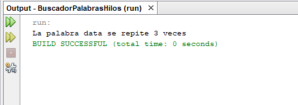
\includegraphics[scale=1.5]{51.jpg}\par} 
		\caption{Salida del primer programa, Actividad 10}\vspace{1cm}
\end{figure}

\textbf{\textit{Solución del segundo programa.}}

\begin{center}
Clase Adquiere.java
\end{center}

\begin{verbatim}
public class Adquiere extends Thread {

    private Control pila;
    private int n, dormir;

    public Adquiere(Control pila, int n, int dormir) {
        this.pila = pila;
        this.n = n;
        this.dormir = dormir;
    }

    @Override
    public void run() {

        try {
            char c;

            for (int i = 0; i < n; i++) {
                c = pila.retirar();
                System.out.println("Envió: " + c);
                sleep((int) (Math.random() * dormir));
            }
        } catch (Exception ex) {
            System.out.println("");
        }
    }
}
\end{verbatim} \vspace{1cm}

\begin{center}
Clase Control.java
\end{center}

\begin{verbatim}
public class Control {

    private char[] pila = null;
    private int tope = 0;
    private boolean lleno = false;
    private boolean vacio = true;

    public Control(int capacidad) {
        pila = new char[capacidad];
    }

    public synchronized void agregar(char c) throws Exception {
        while (lleno) {
            wait();
        }
        pila[tope++] = c;
        vacio = false;
        lleno = tope >= pila.length;
        notifyAll();
    }

    public synchronized char retirar() throws Exception {
        while (vacio) {
            wait();
        }
        char c = pila[--tope];
        lleno = false;
        vacio = tope <= 0;
        notifyAll();
        return c;
    }

}
\end{verbatim} \vspace{1cm}

\begin{center}
Clase Producir.java
\end{center}

\begin{verbatim}
public class Producir extends Thread{
    
    private Control pila;
    private int np, dormir;

    public Producir(Control monitor, int np, int dormir) {
        this.pila = monitor;
        this.np = np;
        this.dormir = dormir;
    }
    
    
    @Override
    public void run(){
        char c;
        for (int i = 0; i < np; i++) {
            c=(char)('A'+i);
            try {
                pila.agregar(c);
                System.out.println("Ingresó: "+c);
                sleep((int)(Math.random()*dormir));
            } catch (Exception ex) {
                System.out.println("Hilo producir"+ex.getMessage());
            }
            
        }
    }
}
\end{verbatim} \vspace{1cm}

\begin{center}
Clase SincronizacionHilosDiplomado.java (main)
\end{center}

\begin{verbatim}
public class SincronizacionHilosDiplomado {

    public static void main(String[] args) {
        // TODO code application logic here
        Control c = new Control(3);
        Producir p = new Producir(c, 6, 1500);
        Adquiere a = new Adquiere(c, 6, 2000);
        p.start();
        a.start();
    }
    
}
\end{verbatim} \vspace{1cm}
\begin{figure}[h!]
		\centering
		{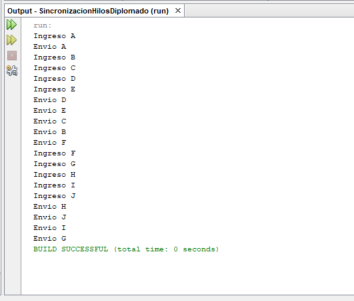
\includegraphics[scale=1]{52.jpg}\par} 
		\caption{Salida del segundo programa, Actividad 10}\vspace{1cm}
\end{figure}

{\raggedright
\subsection{Actividad 11 en clase}
}\vspace{.5cm}

\textbf{Desarrolla un programa Cliente-Servidor utilizando sockets.}\vspace{1cm}

\textbf{\textit{Solución del programa.}}\vspace{.5mm}

\begin{center}
Clase Cliente.java (main)
\end{center}

\begin{verbatim}
public class Cliente extends javax.swing.JFrame implements Runnable {

    public Cliente() {
        initComponents();
        Thread hilo2 = new Thread(this);
        hilo2.start();
    }

    private void btnSalirActionPerformed(java.awt.event.ActionEvent evt) {                                         
        // TODO add your handling code here:
        System.exit(0);
    }                                        

    private void btnEnviarActionPerformed(java.awt.event.ActionEvent evt) {                                          
        try {

            Socket sC = new Socket("localhost", 9999);
            ObjectOutputStream salidaMensaje = new ObjectOutputStream(
						sC.getOutputStream()
						);
            Datos dat = new Datos();
            dat.setIp(ipDestino.getText());
            dat.setMensaje(Mensaje.getText());
            dat.setNombre(nombre.getText());
            salidaMensaje.writeObject(dat);
            AreaTexto.append(Mensaje.getText());
            salidaMensaje.close();

        } catch (IOException ex) {
            System.out.println("Error en la conexión de cliente" + ex.getMessage());
        }
    }
		
    //Encapsular los datos del cliente para enviar a servidor
    public class Datos implements Serializable {

        private String nombre;
        private String ip;
        private String mensaje;

        public String getNombre() {
            return nombre;
        }

        public void setNombre(String nombre) {
            this.nombre = nombre;
        }

        public String getIp() {
            return ip;
        }

        public void setIp(String ip) {
            this.ip = ip;
        }

        public String getMensaje() {
            return mensaje;
        }

        public void setMensaje(String mensaje) {
            this.mensaje = mensaje;
        }
    }
		
    @Override
    public void run() {
        int i = 0;
        try {
            ServerSocket CEscucha = new ServerSocket(9999);
            Socket cliente;
            Datos dat = new Datos();
            while (i == 0) {
                cliente = CEscucha.accept();
                ObjectInputStream flujoEntrada = new ObjectInputStream(
								cliente.getInputStream()
								);
                dat = (Datos) flujoEntrada.readObject();
            }
        } catch (IOException ex) {
            Logger.getLogger(Cliente.class.getName()).log(Level.SEVERE, null, ex);
        } catch (ClassNotFoundException ex) {
            Logger.getLogger(Cliente.class.getName()).log(Level.SEVERE, null, ex);
        }

    }
}
\end{verbatim} \vspace{2cm}

\begin{center}
Clase Servidor.java (main)
\end{center}

\begin{verbatim}
public class Servidor extends javax.swing.JFrame implements Runnable {

    public Servidor() {
        Thread hiloServer = new Thread(this);
        hiloServer.start();
        initComponents();
    }
		
    @Override
    public void run() {
        try {
            ServerSocket ss = new ServerSocket(9999);
            int i = 0;
            while (i == 0) {
                Socket sC = ss.accept();/*
                 DataInputStream mensajeEntrada = new DataInputStream(
								sC.getInputStream()
								);
                 String datoTexto = mensajeEntrada.readUTF();
                 System.out.println("Texto Servidor " + datoTexto);
                 areaTexto.append(datoTexto+"\n");*/

                ObjectInputStream salidaMensaje = new ObjectInputStream(
								sC.getInputStream()
								);
                Datos dat = (Datos) salidaMensaje.readObject();
                System.out.println("Texto Servidor " + dat);
                String name = dat.getNombre();
                String ip = dat.getIp();
                String mensaje = dat.getMensaje();
                System.out.println(name + ip + mensaje);

                TextArea.append(name + ":" + ip + "\n" + mensaje);

                Socket enviaDestinatario = new Socket(ip, 9999);
                ObjectOutputStream paqueteReenvio = new ObjectOutputStream
								(enviaDestinatario.getOutputStream());
                paqueteReenvio.writeObject(dat);
                enviaDestinatario.close();
                sC.close();

            }

            ss.close();
        } catch (IOException ex) {
            Logger.getLogger(Servidor.class.getName()).log(Level.SEVERE, null, ex);
        } catch (ClassNotFoundException ex) {
            Logger.getLogger(Servidor.class.getName()).log(Level.SEVERE, null, ex);
        }
    }
}
\end{verbatim} \vspace{1cm}